\part{Motion Detector}
\paragraph{A Motion Detector is a camera device that uses hardware or software to detect a significant change between scenes and flag that movement has occurred. The first motion detector was invented by Samuel Bagno in the 1950s as a burglar alarm, making use of ultrasonic waves to measure the Doppler change in frequencies to measure movement. Modern day motion detectors make use of the same technology; using infrared to measure changes in heat, or microwave lasers to measure the distance of a scene.\\
Mobile phone's however do not come equipped with microwave lasers nor ultrasonic emitters, and though a significant amount of mobile phones have infra-red sensors and bluetooth radio sensors, the poor resolution of these sensors makes using them as reliable motion detectors somewhat tricky.\\
Modern smartphones of today do often come equipped with camera's whose images can be used to detect motion, but all the processing is done in the software which can be slow. Fortunately smartphones of today are fast enough to handle such image processing, and using lower-level languages such as C and C++ the strain on the phone can be greatly reduced.}

\section{Competition}
\paragraph{Due to the small community of Maemo users, there are not many apps of this nature on the platform and thus not much competition at all.}

\section{Software Battles}
\paragraph{To start a basic motion detector, the very least that I would need to do is take one frame and subtract it from another to see the difference. To do this I would need to store every pixel value in an array for each image and then perform a sweep over both arrays to compare their pixel values. There must be imaging libraries that I could use that would greatly facilitate such imaging techniques. But first I would need to be able to take a single photo.....}

\subsection{QtMobility vs Gstreamer vs FCam}
\paragraph{\bf{QtMobility}}
\paragraph{QtMobility is a Qt library that enabed developers to have access to standard mobile functionality such as messaging, contacts, multimedia, and camera.  The camera is contained within a QCamera widget and simple calls can be made to the imaging device.
\\Unfortunately the official stable version v1.1 had camera support for Symbian and Meego(Harmattan), but not Fremantle. There was an unstable version 1.2 which included Fremantle support, but once I had installed libqtm-dev\_1.2 on the rootstrap device, and tried to use the QCamera element from within a C++ class it did not work. This is because the QCamera element has to be accessed through QML, which would be doable but would not be optimized for speed. For this reason I dropped QtMobility.
}
\pagebreak %encourage
\paragraph{\bf{GStreamer}}
\paragraph{GStreamer is an open source multimedia framework that is already native to Fremantle since it is the library that the default mediaplayer uses and so would reduce the dependencies of my application. GStreamer makes use of pipelining, byt connecting a number of elements in an ordered fashion so that the output (source) of one element is fed into the input(sink) of another element and so on until it reaches the final element which is usually a file or a network stream.
\\\\A previous app of mine was Gstreamer based and a typical command from it would be:
}
\begin{verbatim}
	      gst-launch v4l2src device=/dev/video0 ! \
	      videoscale ! video/x-raw-yuv, width=320, height=240 ! \
	      ffmpegcolorspace !  jpegenc 80 ! \
	      tcpserversink host=192.168.1.101 port=9000
\end{verbatim}
\paragraph{This pipes the video-for-linux(version2) camera source into a video scaling element, into a raw video stream of defined height and width, into an element that convert the pixel color depths to type ffmpeg color sizes, into an element that encodes the raw stream into mjpeg format with a quality of 80\%, which then pipes it into a tcp server element which broadcasts to the specified host and port.
\\On the recieving side, a gstreamer pipe would need to reverse the order of the elements (i.e. recieve from tcpserver, feed it into a jpeg decoder, and then specify an output window or file sink.
\\Gstreamer is very well developed, and has a Good, Bad, and Ugly heirarchy of stable to unstable plugins that can be used to enable a wide array of different multimedia functionalities and formats.
}
\paragraph{Despite the speed and efficient usage of system resources, GStreamer has an extremely involved API but is difficult to work with since it is prone to cascading errors due to the every element being dependant on the previous element to function. An example of the C++ implementation of the same code as above is shown in the appendix.}


\paragraph{\bf{FCam}}
\paragraph{FrankenCamera (or FCam) is a very easy to use open-source C++ API for controlling digital cameras.  The FCam architecture was developed as a joint reasearch project between Stanford Computer Graphics and Nokia's Research Center for controlling the N900's camera, but has since been used to run their own F2 camera built in their labs\cite{fcamdoc}. Normally camera architectures are not so easily accessible and it is very fortunate that FCam chose the N900 to develop on.
\\The FCam API is split into 4 components:}
\begin{enumerate}
\item[Device]{The camera device consists of a Lens, a Flash and other different devices. FCam has object classes for each of these with various functionlity enabled.}
\item[Shot]{The shot object holds typical parameter settings such as exposure time, frame time, white balance, and gain for capturing and processing a single image. It is applied to the sensor object.}
\item[Sensor]{The sensor object listens for calls for capture, and outputs a frame by performing all the image pipelining in it's own thread. Once pipeline exits (or the thread terminates) the sensor is ready to be configured for the next frame.}
\item[Frame]{Frames can be accessed from the sensor by calling the getFrame() function which performs blocking on any pending shots. The ease of API is shown here, as this is the \it{only} blocking call in the entire API.}
\end{enumerate}

\begin{wrapfigure}{R}{0.5\textwidth}
	\vspace{-40pt}
	\begin{center}
		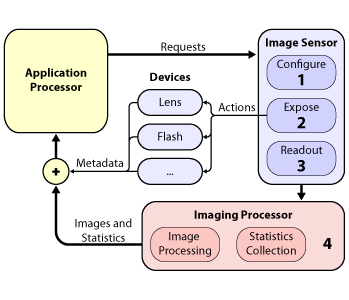
\includegraphics[width=0.5\textwidth]{images/fcam_arch}
	\end{center}
	\vspace{-20pt}
	\caption{FCam Architecture}
\end{wrapfigure}
\paragraph{It has an extermely simple API, since all the user has to do is set the shot parameters, call a new frame, and grab the image from the frame. This can be called any times in succession using the same parameters with comparitavely little lines of code.\\
Despite being a relatively small project, the API was extremely detailed and had many examples that I could adopt. For these reasons, FCam was the acrhitecture used for the developement of this project.
\\
To use it, I had to add an -lfcam dependency to the LIBS+= heading in the .pro file, and fcam-dev\_1.2.deb had to be installed to the rootstrap device.
\\
FCam has different image sizes depending on the colorspace of the frame that it is being extracted from. For example RAW formats only allow an aspect ratio of 4:3 (2592x1968, 1296x984, 648x492, ...160x120). However using RAW images may be better for precise image processing, but the memory it uses has a lot of overhead and for frequent repetitive use it is not very practical.}
\paragraph{Instead the FCam::UYVY colorspace was adopted which captures the image using three components: Y, U(Cb), and V(Cr). 
Images in this format allow subsampling to reduce the color band resolution (U and V) with a constant brightness (Y) without affecting the image quality discerniable to the human eye. This is because the human eye percieves changes in colour much less significantly than changes in brightness. UYVY format adopts the 4:2:2(Y:U:V) scaling system, where Y is sampled at every pixel and U and V are sampled at every second pixel horinzontally on each line. This greatly reduces the memory size of the image and speeds up processing with very little difference in quality.\\
Supported UYVY image sizes are: (2592x1968, 1280x960, 800x600, 640x480, 320x240, 160x120)}

\subsection{OpenCV vs CImg}
\subsubsection{OpenCV}
\paragraph{Now that I had my camera driver configured, I needed to choose an appropriate image library to perform the processing. Technically I could have written my own library class to perform the simple image subtraction and addition functions that I wanted, but there may have been more to offer down the line and I wanted to see what was available}
\paragraph{OpenCV and CImg are both common imaging libraries for C, C++, and Python, for use with real-time image proccessing. 
Both are used widely in computer vision applications, and both contain approximately the same core capabilities, though OpenCV has more extraneous features.}
\paragraph{The Open Source Computer Vision Library (or OpenCV) was developed by Intel for use with computer vision applications, but since was dropped and is now maintained by Willow Garage and Itseez.
\\OpenCV comes with many useful functions for motion detection: image subtraction, image averaging, normalising, and even its own method for tracking movement. It has an image format called IPLImage and inorder to preform operations I have to convert from FCam's relatively unknown Fcam::Image format to IPLImage. This proved difficult.
}
\paragraph{The FCam Image format is made up of:
FCam::Image::Image(
     int width,
     int height,
     Imageformat f,
     unsigned char* data,
     int srcByesPerRow
)
The IPLImage has BGR channel order (i.e the first channel is blue, second is green, third is red. This is different from standard RGB formats). I attempted to convert to a grayscale IPLImage by doing:}
\lstinputlisting[title=\textbf{Source Code: IPLconvert.cpp}]{Code/API_Examples/IPLconvert.cpp}
\paragraph{as taken from http://www.cs.cornell.edu/courses/cs4670/2010fa/projects/p1/codes/project1.tar.gz\\
This took a reference to the FCam's Frame, extracted the image from it, and attempted to convert it into an unsigned 8-bit gresycale IPL image with 1 color channel. The unsigned 8-bit image would be limited to 0-255 range.\\
Unfortunately several problems were encountered and almost three days were lost trying to get to the bottom of it:}
\paragraph{
A Maemo port of openCV does exist for Fremantle \cite{libcv} but despite installing libcv, libcv-dev, and many of it's dependencies (libcvcore, libhighgui) the SDK would complain about many missing dependencies when building the application. The culprit turned out to be missing dependencies for libhighgui-dev, but this was false since running a quit dpkg -L <dependency\_name> confirmed that the dependency was indeed installed. At one stage I copied my entire /usr/lib directory from the phone to the rootstrap but it would still fail when trying to build.\\
A few hours of trawling through the Maemo reading lists came up with a bug report \cite{highgui-dev} from the original maintainer claiming a bug within the build system.\\
For this reason OpenCV had to be abandoned and a new image processing library had to be used.
}
\subsubsection{CImg}
\paragraph{CImg was suggested by my project supervisor after we discussed the bugs I had been experiencing. CImg is relateivly bug free since it does not exit in any packaged form. In fact all the functions and image processing capabilities are contained within a single 40,000 lined header file coming up to 2.54MB in size. \\Despite the jaw-dropping overhead of including this file in development process, Qt only had to parse the functions within it once and it was set to go.\\
Another bonus is that it removes a dependency from the project, and makes it all that much more portable. One thing I had to do first was to convert from FCam to CImg.
\\The CImg constructor is formed of: 
CImg(const unsigned int width,
     const unsigned int height,
     const unsigned int size\_z=1, //depth
     const unsigned int size\_c=1 //spectrum
)
And to construct a CImg, all one has to do is call CImg<T> name; where T is the type or size of each pixel value, and name is the name of the image. So for an image that that has 256 colorspace, T = unsigned char = 8bit.
In CIMG, the color channels are in RGB format. OpenCV's IPLImage only supports up to 4 color channels but CImg supports up to any number and this provided a source of initial confusion for me:
http://sph2grid.googlecode.com/svn-history/r14/trunk/CImg/plugins/cimg\_ipl.h:\\
Using the same format as the cornell code I attempted to make:}
\lstinputlisting[title=\textbf{Source Code: IPLconvert.cpp}]{Code/API_Examples/CImgConvertBad.cpp}
\paragraph{This wasn't able to produce a consistent image (or any image at all) and I had to play around a wide variety of pixel values:}
\begin{verbatim}
//MAGENTA
newimg1(i,j,0, 0) = pixels[0]; //red
newimg1(i,j,0 ,1) = pixels[1]; //green
newimg1(i,j,0, 2) = pixels[2]; //blue;
//
//BLACK IMAGE
newimg2(i,j,0, 0) = pixels[0]/255; //red
newimg2(i,j,0 ,1) = pixels[1]/255; //green
newimg2(i,j,0, 2) = pixels[2]/255; //blue;
//
newimg3(i,j,0) = pixels[0]; //red
newimg3(i,j,1) = pixels[1]; //green
newimg3(i,j,2) = pixels[2]; //blue;
//
newimg4(i,j,0) = pixels[0]/255; //red
newimg4(i,j,1) = pixels[1]/255; //green
newimg4(i,j,2) = pixels[2]/255; //blue;
//GREEN
newimg5(i,j,32, 0) = pixels[0]; //red
newimg5(i,j,32, 1) = pixels[1]; //green
newimg5(i,j,32, 2) = pixels[2]; //blue;
//BLACK IMAGE
newimg6(i,j,32, 0) = pixels[0]/255; //red
newimg6(i,j,32, 1) = pixels[1]/255; //green
newimg6(i,j,32, 2) = pixels[2]/255; //blue
\end{verbatim}
\paragraph{The idea was that by specifying the (i,j) coordinates of the new image and grabbing the pixel values from the FCam image and sticking it into (i,j) coordinates of the new CImg. I attempted to divide by 255 in some of the tests because I wasn;t sure how large the FCam::Image was, and this was my idea of normalizing it. I later realised that the pixel values were already normalized to 8-bit values and that dividing by 255 limited the CImg to \{0,1\} values would ultimately produce a black image.}
\paragraph{By digging around through the source of the original fcam application for the N900, I was able to find a function that converted FCam by accessing the image data and reading from it:}
\lstinputlisting[title=\textbf{Source Code: CImgConvertFcam.cpp}]{Code/API_Examples/CImgConvertFcam.cpp}
This resulted in images that looked like this:
\begin{wrapfigure}{R}{0.3\textwidth}
	\vspace{-20pt}
	\begin{center}
		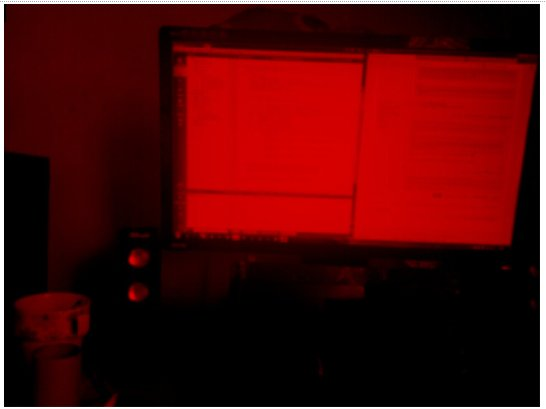
\includegraphics[width=0.3\textwidth]{images/redbuffer1}
	\end{center}
	\vspace{-20pt}
	\caption{Very red image.}
\end{wrapfigure}
\paragraph{
A similar image would appear using imgBuffer[1] instead of imgBuffer[0], and I didn't understand why until I looked up CImg's documentation and realised that out of the 32 channels I was initialising, the first channel is red and that was the only channel I was writing to.
That is, for a greyscale image from 0-255 at pixel i,j - I was sticking it into CImg\{Red,0,0,0,0....32 times.\}, and thus ending up with a red image.
\\
Once I limited CImg to 1 color channel (i.e. black and white) then I got my desired image as shown by the real and greyscale comparison below:
}
\begin{wrapfigure}{R}{0.3\textwidth}
	\vspace{-20pt}
	\begin{center}
		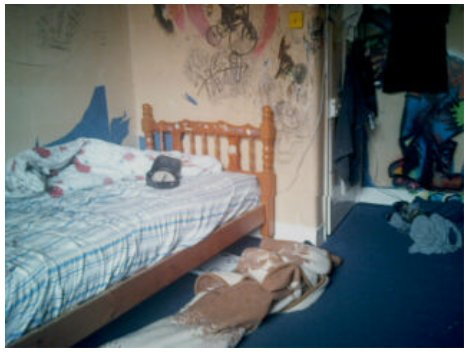
\includegraphics[width=0.3\textwidth]{images/realbuffer2}
	\end{center}
	\vspace{-20pt}
	\caption{Image saved by FCam}
	\vspace{10pt}
	\begin{center}
		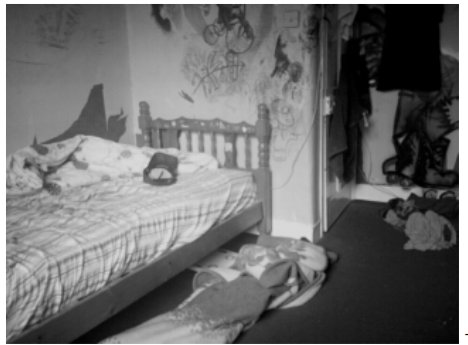
\includegraphics[width=0.3\textwidth]{images/blackbuffer3}
	\end{center}
	\caption{Image saved by CImg}
	\vspace{-20pt}
\end{wrapfigure}

\subsection{ImageMagick vs FFMpeg vs VLC vs Mencoder}
\paragraph{Now that the image processing side of this was underway, I needed a program that could convert a series of images into a movie format so that when the user returns to their motion detector, they can watch all the highlights in the movie file over the course of a few seconds rather than having to flit through each individual image.
}
\paragraph{Imagemagick is an open-source image software library for processing images. It can perform much of the same functions and CImg and OpenCV, but it was not considered as a suitabe image processing library because the development package had not been released for Maemo and compatibility was a concern. There is, however, a imagemagick package for Maemo that performs the functions from commandline and so accessing its functions would not be a problem if I was resigned to the fact that I would be calling a system process from Qt. CImg has good compatibility with Imagemagick since it's convertToJPEG command actually calls the 'convert' module of Imagemagick.\\
According to the documentation, to convert a series of jpegs to a movie format, all one has to do is call:
'convert -delay <frametime> input\_jpegs\_*.jpg output\_movie.mpg'\\
But this failed with Maemo specific errors:}
\begin{verbatim}
Nokia-N900:/home/user/MyDocs/DCIM/MISC\# convert -delay 20 -monitor timelapse-0000*.jpg movie.mpg
load image[timelapse-000001.jpg]: 479 of 480, 100\% complete
load image[timelapse-000002.jpg]: 479 of 480, 100\% complete
...
load image[timelapse-000015.jpg]: 479 of 480, 100\% complete
mogrify image[timelapse-000015.jpg]: 9 of 10, 100\% complete
Composite/Image[movie.mpg]: 479 of 480, 100\% complete
..
Composite/Image[movie.mpg]: 479 of 480, 100\% complete
Save/Image//var/tmp[magick-XX9TmsAd7.jpg]: 479 of 480, 100\% complete
..
Save/Image//var/tmp[magick-XX9TmsAd63.jpg]: 479 of 480, 100\% complete
convert: Empty input file `timelapse-000001.jpg' @ error/jpeg.c/EmitMessage/233.
..
convert: Empty input file `timelapse-000010.jpg' @ error/jpeg.c/EmitMessage/233.
Nokia-N900:/home/user/MyDocs/DCIM/MISC\# 
\end{verbatim}
\paragraph{so I was not able to use imagemagick on the device. This is perhaps a good thing since the imagemagick suite is very large and would be a hefty dependency to add to my project
}
\paragraph{FFmpeg was my next and most immediate option - I have used it countless times before to convert movie files and I have found it's libavcodec library a powerful and useful tool in the past. FFMpeg is one of the most popular free multimedia frameworks around, supporting every single codec and format under the sun. It has a fast release time too and when a new format is released it is not usually a long wait before ffmpeg has a supporting library for it. FFmpeg is primarily used to stream, convert, decode, mux, demux and transcode video files into different formats, but is not used for computer vision.\\
For converting a series of images to a movie file the documentation states that one has to call:\\
'ffmpeg -i name\_of\_files\_\%05d.jpg -y movie.mpg -r fps'\\
It is key to note here that the y flag overwrites any output file that already exists, and that the frames-per-second flag '-r' must be placed at the end. The \%05d just notifies FFmpeg that the format for the image files are padded by zeros by up to 5 digits.\\
Despite using different arrangements and different flags, this only partially worked, as the images would be compiled into a movie, but the framerate flag was temperamental and sometimes ignored.\\
Additionally ffmpeg does not come installed as default by the device, since gstreamer is main multimedia framework used by the mediaplayer and this would also be a needlessly large dependency to have for my project
}
\paragraph{VLC is a comparitavely new open-source mediaplayer which can also perform transcoding, streaming, muxing and the same functions as FFMpeg. In fact alot of its codecs are actually taken from the ffmpeg project (e.g. libavcodec), but it also contains a lot of its own.\\
VLC has only been very recenly ported to Maemo and is accessed by adding user Qole's repository to the /etc/apt/sources.list. It is very incomplete, lacking a decent GUI, but it has a working backend. Unfortunately nowhere in the documentation does it mention being able to convert a series of jpegs to a movie file and I soon had to abondon VLC too.\\ This is probably for the best since VLC is not available in the main repositories and users would find it hard to access. This leaves...}
\paragraph{Mencoder is yet another multimedia framework released under GPL, and comes as a module with mplayer, a very stable open-source media player that comes with all the codecs and formats that mencoder can use.\\
To convert a series of images to a movie file one simply has to call:\\
'mencoder "mf://path/to/images*.jpg" -mf fps=<fps> -o movie.mpg -ovc lavc -lavcopts vcodec=mjpeg'\\
which specifies the that libavcodec is to be used, the framerate and also that the output videocodex should be mpeg format.
\\Mencoder is also not pre-installed with the device, but many Maemo users do tend to install it first chance they get due to the default Media Player's poor support for certain MPG formats, this is by far the most convenient of the four video processing libraries to use and best of all it actaully works.
}
\section{Image Processing Techniques}
\paragraph{A motion detector works on the basic priniciple that there there exists some drastic difference between two images where motion has occred and motion has not occured. One way to see this represenation is to subtract one frame from another and look for the leftover pixels. Pixels where the image hasn't changed will have the same pixel value and will thus cancel each other out, whereas images where there is a difference between pixels at the same location will have values greater than zero. In the case of unsigned chars, any negative pixels will naturally wrap around and becomes high pixel values (white).}
\subsection{Subtraction}
\paragraph{Subtraction is the technique that performs this, and CImg handles this operation using the basic numerica operator '-', so that for example: CImg<T> diff = CImg<T>A - CImg<T> B;
}
\begin{wrapfigure}{R}{0.3\textwidth}
	\vspace{-20pt}
	\begin{center}
		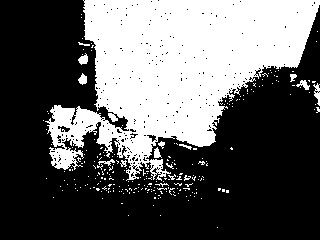
\includegraphics[width=0.3\textwidth]{images/subG}
	\end{center}
	\vspace{-20pt}
	\caption{Image subtraction between two consecutive frames where the scene has changed inbetween}
	\vspace{10pt}
	\begin{center}
		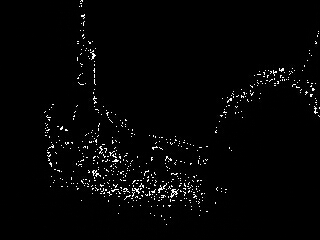
\includegraphics[width=0.3\textwidth]{images/subF}
	\end{center}
	\vspace{-20pt}
	\caption{Image subtraction between two consecutive static frames where no movement has occured}
\end{wrapfigure}
\paragraph{The images above were normalised to 2 discrete \{0,1\} values and then multiplied by 255 so that the 'hot pixels' could be viewed with the human eye. As you can see from the top figure, the whiteness indeicates that there was a significant difference between frames and so that one of the images had pixel values vastly greater than the other -- indicating a change in the scene.
\\For the bottom image it can be seen that there is very little difference exists between the frames, yet you can almost quite clearly makeout the edge of the objects between the frames (a computer screen and speaker). Neither the speaker, the monitor, nor the camera moved between those two images but nonetheless a small difference was detected.\\
This served as my first model for image detection by performing a small test to see how many of these sparse white pixels are detected for static frames. This would then serve as the basis for a threshold, so that any subtracted frames that are significantly above this threshold are flagged as 'movement' frames and those below or up to the threshold 
are not.}
\underline{Experiment 1: Determining a suitable threshold for subtracted images}
\paragraph{To find a suitable threshold I used the following pseudocode to determine a threshold for a static frame:\\\\}
\lstinputlisting[title=\textbf{Source Code: subtract1.pseudo}]{Code/pseudo/subtract1.pseudo}
\paragraph{It essentially grabs an image and subtracts it subtracted one image from another and totalled up all the pixels with a value greater than zero. This gave the following table of results:}
\begin{center}
\begin{table}
	\begin{tabular}{| c | l | l | l | l | l | }
\hline
\multicolumn{6}{|c|}{\bf Non-Zero Counts from Subtracted Images} \\
\hline
\bf Test	&\bf Scene 1	&\bf Scene 2	&\bf Scene 3	&\bf Scene 4	&\bf Scene 5	\\ \hline
1	&30747	&47298	&37881	&18801	&678\\
2	&9067	&9129	&33326	&7645	&8488\\
3	&798	&35861	&17947	&6433	&444\\
4	&3841	&30449	&8273	&23614	&13385\\
5	&34379	&25246	&6303	&41523	&23474\\
6	&9144	&256	&14960	&31458	&25138\\
7	&333474	&312598	&771731	&33779	&725415\\
8	&34488	&2676	&14522	&1256	&12165\\
9	&36351	&12497	&472	&1036	&18955\\
10	&6133	&23077	&12343	&31430	&25410\\ \hline
\bf Average	&49842.2	&49909	&91776	&19698	&85355\\ \hline
	\end{tabular}
	\label{tab:sub1}
\end{table}
\end{center}
\paragraph{as shown in \cref{tab:sub1} the Average white pixel count is extremely high and varies greatly from scene to scene. Setting a threshold of less than 90000 would work for the five different scenes tested in my experiment, but there’s no gauruntee that the fluctuation between frames would not be higher than 90000 for another scene. \\
So Why is there so much fluctuation? For one, the average pixel values of one scene can be radically different to another scene. If the average pixel value for Scene1 is 45 and the average pixel value for Scene2 is 90, then assuming that the ambient light in a scene is decreased by 10\%, then this would result in:\\
Scene1:  45-40.5 = 4.5, and Scene2: 90-81 = 9 --- which are proportionately different counts for the same reduction in ambient light.\\
 }
\paragraph{My second attempt addresses the proportion problem, and inserts extra code into lines 5 and 7.}
\lstinputlisting[title=\textbf{Source Code: subtract2.pseudo}]{Code/pseudo/subtract2.pseudo}
\paragraph{Here it normalise the current frame into [0,1] binary colorspace after taking it. It then performs the subtraction, but this subtraction may result in pixel values greater than 1 due to overflow (i.e. 0-1 = -1 = 255 for 8-bit unsigned pixel), so a normalisation is performed on subtracted image as well. \\
This results in non-zero counts of subtracted images that are far more stabler as shown in the table}
\begin{center}
\begin{table}
	\begin{tabular}{| c | l | l | l | l | l | }
\hline
\multicolumn{6}{|c|}{\bf Non-Zero Counts from Subtracted Images} \\
\hline
\bf Test	&\bf Scene 1	&\bf Scene 2	&\bf Scene 3	&\bf Scene 4	&\bf Scene 5	\\ \hline
1	&24272	&18049	&19899	&19746	&18833\\
2	&23691	&21275	&19730	&21381	&20744\\
3	&20607	&23001	&19261	&19711	&24503\\
4	&19134	&22938	&23231	&21930	&21096\\
5	&22282	&20143	&19616	&24927	&22492\\
6	&23242	&18886	&19865	&20627	&21682\\
7	&23769	&24513	&23851	&23883	&20993\\
8	&21132	&22961	&23835	&24969	&23704\\
9	&22978	&23870	&21845	&21534	&18847\\
10	&22031	&22578	&18717	&24348	&20265\\ \hline
Average	&22313.8	&21821	&20985	&22306	&21315.9	\\ \hline
	\end{tabular}
	\label{tab:sub2}
\end{table}
\end{center}
\paragraph{Using the results from this table I decided to set a threshold of less than 26000 (i.e. a white-pixel count of less than 26000 will NOT trigger a movement flag. Anything above will). 
\\However this threshold was purely for 320x240 images. At that stage I had not considered using different image sizes  for motion detection, but since FCam supported larger sizes I decided to test thresholds for these too, expecting a linear relationship between image size and non-zero count.
\\For this experiment I repeated the same experiment for the five different image sizes, but have only included the average counts per }





%\\EXPERIMENT 1: Finding the threshold
%\\There are two factors that would affect the threshold: Image size and thats it haha
\subsection{Running Average}
\paragraph{The running average method is the process of adding up the pixel values of several frames and storing them in an accumulator. This accumulated image is then normalised and the image is converted into regular colorspace. This can be done either by dividing the pixel values by the number of frames added, 
}
\footnote{CImg facilities this very easily by using standard operators to perform operations over all pixel values.\\ E.g.  CImg<T2> average =  (CImg<T1>one + CImg<T1> two + CImg<T1> three) / 3; // Where: sizeof(T2)>sizeof(T1)} 
\paragraph{
or by simply normalising the image in [0,255] colorspace.
\\It should be noted once again that greyscale image sizes are unsigned chars with a maximum and minimum values from 0 to 255, so appending a series of pixel values will result in in values that overflow this range. For this reason, the accumulator needs to have pixel sizes that can contain accumulated pixel sum amounts.
}
\begin{wrapfigure}{R}{0.3\textwidth}
	\vspace{-20pt}
	\begin{center}
		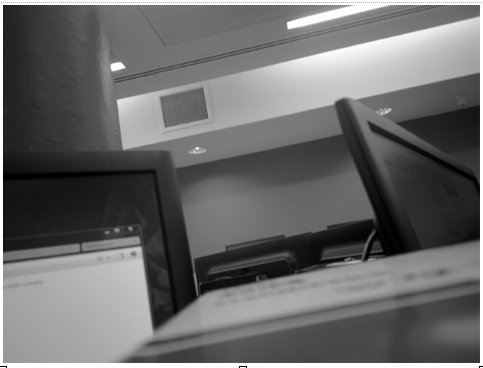
\includegraphics[width=0.3\textwidth]{images/accumstatic}
		\label{accumst}
	\end{center}
	\vspace{-20pt}
	\caption{10 frame accumulation for static scene}
	\vspace{10pt}
	\begin{center}
		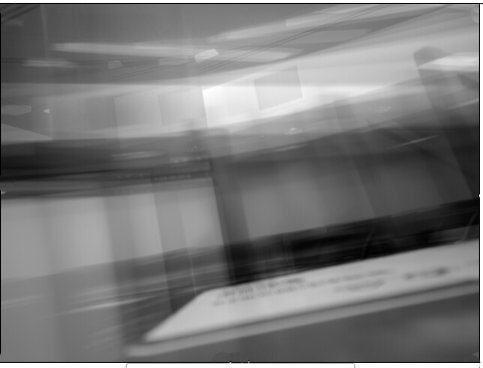
\includegraphics[width=0.3\textwidth]{images/accumdynamic}
		\label{accumdy}
	\end{center}
	\vspace{-20pt}
	\caption{10 frame accumulation for dynamic scene}
\end{wrapfigure}
\paragraph{As shown in ~\cref{accumst} a static scene shows very little difference from one scene to the next so that the image is coherent. For a dynamic scene, \cref{accumdy} shows a wildly different image with traces of many different scenes superimposed.
\\This approach has a lot less overhead than the subtraction method since it doesn’t require the program to subtract every frame with the previous. It also introduces the concept of having a background or reference, since by the subtraction method of motion detection we would have no knowledge of the background since we would only be comparing two temporally adjacent frames.
}

\paragraph{Results}
\paragraph{Analysis}
\subsection{Determining a Threshold for Detection}
\paragraph{Counting white pixels (ineffective by itself, scatter}
\paragraph{Noise}
\subparagraph{Thermal Noise, CCD clocking up/down}
\subparagraph{Oversaturation, filtering, compression}
\subsection{Image Morphology}{Noise Removal}
\subsubsection{Kernel Mask}
\paragraph{Diamond,Square}
\subsubsection{Erode, Dilate}{Open/Close}
\section{Threads}
\subsection{Camera Thread}
\subsubsection{Signal/Slots}
\subsubsection{QImage, QPixMap, and CImg}
\subsection{Email Thread}
\paragraph{Setting up an SMTP Server}
\paragraph{Existing Frameworks}{QTCPSocket from version 3.x}
\paragraph{Adoption of mailcmd}
\subsection{Multiple Inheritance}{QObject and QThread}
\subsection{Optimisations/Error Proofing}
\subsubsection{Kernel Compatibility}
